\documentclass[dvipdfmx]{jarticle}
\usepackage{graphicx}
\usepackage[top=30truemm,bottom=30truemm,left=25truemm,right=25truemm]{geometry}
\usepackage{listings,jvlisting}
\usepackage{url}

\lstset{
  basicstyle={\ttfamily},
  identifierstyle={\small},
  commentstyle={\smallitshape},
  keywordstyle={\small\bfseries},
  ndkeywordstyle={\small},
  stringstyle={\small\ttfamily},
  frame={tb},
  breaklines=true,
  columns=[l]{fullflexible},
  numbers=left,
  xrightmargin=0zw,
  xleftmargin=3zw,
  numberstyle={\scriptsize},
  stepnumber=1,
  numbersep=1zw,
  lineskip=-0.5ex
}

\makeatletter
\newcommand{\subsubsubsection}{\@startsection{paragraph}{4}{\z@}%
  {1.0\Cvs \@plus.5\Cdp \@minus.2\Cdp}%
  {.1\Cvs \@plus.3\Cdp}%
  {\reset@font\sffamily\normalsize}
}
\makeatother
\setcounter{secnumdepth}{4}

\begin{document}
\begin{titlepage}
    \begin{center}
        {\huge 情報科学実験C 期末レポ―ト}
        \vspace{180pt}\\
        \begin{tabular}{rl}
            氏名 & 山久保孝亮\\
            所属 & 大阪大学基礎工学部情報科学科ソフトウェア科学コース\\
            メールアドレス & u327468b@ecs.osaka-u.ac.jp\\
            学籍番号 & 09B22084\\
            提出日 & \today\\
        \end{tabular}
    \end{center}
\end{titlepage}
\section{課題11で作成したプログラムの動作仕様}
課題11では,乗算を行うプログラムを実装した.このプログラムの仕様は以下の通りである.
\begin{itemize}
  \item 掛けられる数と掛ける数は,FPGAボードから入力を行う.どの番地に何が格納されるかは,以下の表1の通りである.
  \begin{table}[h]
    \centering
    \begin{tabular}{|c|c|}
      \hline
      番地 & 格納される内容\\\hline
      8000 & 掛けられる数を格納する.乗算実行後も値は変化しない.\\\hline
      8001 & 掛ける数を格納する.乗算実行後は0となる.\\\hline
      8002 & 掛けられる数と掛ける数に,いくつ負の数が含まれるかを格納する.\\\hline
      8003 & 乗算の実行結果を格納する.結果が負の数なら負の値が格納される.\\\hline
    \end{tabular}
    \caption{各番地に格納される内容}
  \end{table}
  \item まず最初に掛けられる数の入力を行う.掛けられる数はKEY0を押下することでその値が確定する.
  \item 次に掛ける数の入力を行う.掛ける数はKEY1を押下することでその値が確定する.
  \item KEY1を押下し,掛ける数を確定させた後すぐに掛け算の処理が実行される.
\end{itemize}
\section{課題12,13,14で追加した命令の実装方法}
課題12,13,14で追加した命令は,シフト命令である.以下にその仕様を記述する.
\begin{table}[h]
  \centering
  \begin{tabular}{|c|c|c|c|c|}
    \hline
    命令 & オペランド & サイズ & コード & 動作\\\hline\hline
    SLL & num & 1word & 11000001(C1) & IP ← IP+2,A←A<<num(C,Z)\\\hline
    SRL & num & 1word & 11000010(C2) & IP ← IP+2,A←A>>num(C,Z)\\\hline
    SLA & num & 1word & 11000011(C3) & IP ← IP+2,A←A<<num(C,Z)\\\hline
    SRA & num & 1word & 11000100(C4) & IP ← IP+2,A←A>>num(C,Z)\\\hline
  \end{tabular}
  \caption{追加した命令の仕様}
\end{table}
\\上記の命令は,以下の手順に従って実装を進めた.
\begin{enumerate}
  \item ALU内での処理の追加
  \item ALUのデータパスの変更
  \item 外部出力用ジョンソンカウンタを追加
  \item 各信号の条件を変更する.
\end{enumerate}
以下で,これらの詳細について述べる.
\subsection{ALU内での処理の追加}
今回のシフト命令はALU内で演算を実行することにした.ALU内ではmodeALUの値によってfoutに格納される値が決定されるため,modeALUにシフト命令の場合を追加
した.追加後のmodeALUの信号割り当ては以下のようになる.\clearpage
\begin{table}[h]
  \centering
  \begin{tabular}{|c|c||c|c||c|c||c|c|}
    \hline
    0000 & A+B     & 0100 & not A & 1000 & not B & 1100 & SLL\\\hline
    0001 & A-B     & 0101 & A+1    & 1001 & B+1   & 1101 & SRL\\\hline
    0010 & A and B & 0110 & A-1    & 1010 & B-1   & 1110 & SLA\\\hline
    0011 & A or B  & 0111 & 未使用 & 1011 & 未使用 & 1111 & SRA\\\hline
  \end{tabular}
  \caption{modeALU信号割り当て}
\end{table}
また,具体的な処理方法としては,2.2で記述する通りレジスタCの値をALU内で使用できるようにしたため,シフト命令のオペランドの値をCに格納する.このとき,
Cに入る値は1から7までである.この条件の下で,Cの値を利用して以下の二つを行う.
\begin{itemize}
  \item 実際にレジスタAに格納されている8bitの値を即値の数だけシフトする.具体的には,
  \item ゼロフラグとキャリーフラグについて処理する.具体的には,
\end{itemize}
\subsection{ALUのデータパスの変更}
ALU内でシフト命令を実行する際に,即値で入力される値をALU内で使用する必要がある.レジスタBに即値の入力を格納して処理を行うこともできるが,この場合シ
フト命令を実行するとレジスタBに保持していた値が消失するという仕様になってしまう.\\
このため,新たにALUにレジスタCを入力として追加し,レジスタCに即値の入力の値を格納した.これにより,保持していた値が消失するという問題を解消することが
できた.変更後のデータパスは以下の図1のようになる.
\begin{figure}[h]
  \centering
  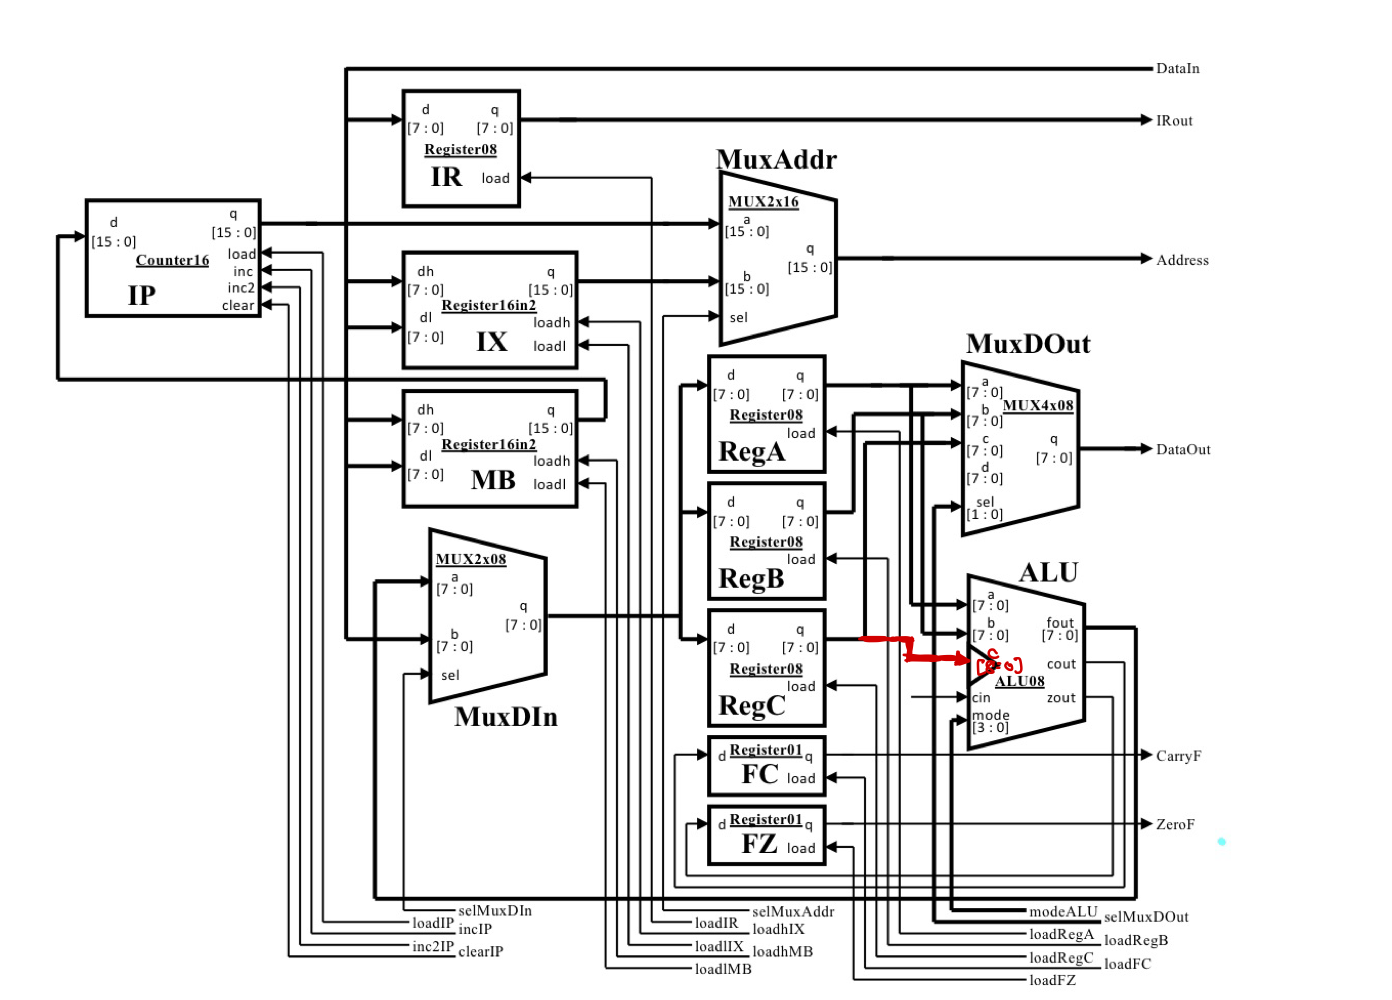
\includegraphics[width = 8cm]{improvedatapath.png}
  \caption{変更後のデータパス}
\end{figure}
\\この図の赤い矢印が,今回追加したレジスタCからALUへのデータパスに対応する.
\subsection{外部出力用ジョンソンカウンタを追加}
シフト命令を実行する際の外部出力用ジョンソンカウンタとして以下を追加した.
なお,内部出力用ジョンソンカウンタはqJCintCと状態数が同じであったためそれを再利用した.
\subsection{各信号の条件を変更する}
2.3の外部出力用及び内部出力用ジョンソンカウンタの追加に応じて,各信号の条件の変更を行った.
\section{工夫点}
\subsection{課題11}
課題11では,掛けられる数と掛ける数を確定させる際に使用するKEYの種類を変更するという工夫を行った.この工夫を行わず,掛けられる数と掛ける数をどちらもKEY0
で値を確定させてしまうと,掛けられる数のみを確定させるつもりが,クロック周波数が早く,掛ける数も同時に確定させてしまうためである.この問題に対する改善策
として,私は掛けられる数を確定させるときはKEY0を,掛ける数を確定させるときはKEY1を使用することにより,クロック周波数が大きいことの影響を受けない設計とす
ることができた.
一方,これ以外の改善策として,JUMP命令を用いて,何も処理しないループをクロック周波数に合わせて十分時間行うという方法が考えられた.しかし,この方法だとJU
MP命令を用いるため,プログラムに変更を加えた場合アドレスの変更を行う必要がある.一方,KEYの種類を変更する方法では,どのKEYを使用してもFFFE番地の値が変更
されるだけであるため,アドレスの変更を行う必要がない.また,SUBA命令などを用いたゼロフラグの情報を活用すれば掛ける数と掛けられる数でほぼ同じプログラムで
実装することができるため,可読性が高まる.
\subsection{課題12,13,14}
課題12,13,14の工夫点は2.1で述べた通り,レジスタBを即値の入力の格納先として使用するのではなく,新たにデータパスを設定しレジスタCを使用した点である.
\section{拡張課題}
\subsection{拡張課題a-1:最大公約数を求めるプログラム}
最大公約数を求めるプログラムの仕様は以下の通りである.
\begin{itemize}
  \item レジスタAに格納されている数値の方がレジスタBに格納されている数値よりも大きい.
  \item 各番地の格納内容は以下の通りである.
  \begin{table}[h]
    \centering
    \begin{tabular}{|c|c|}
      \hline
      番地 & 格納内容\\\hline\hline
      8000 & ユークリッドの互除法における,割る数(計算用)\\\hline
      8001 & ユークリッドの互除法における,余り(計算用)\\\hline
      8002 & レジスタに格納された数値の最大公約数(結果)\\\hline
    \end{tabular}
    \caption{各番地に格納される内容}
  \end{table}
\end{itemize}
最大公約数を求めるプログラムは,以下の手順にしたがって処理を実装した.
\begin{enumerate}
  \item 
\end{enumerate}
\subsection{拡張課題a-2:最小公倍数を求めるプログラム}
\subsection{拡張課題b:演算機の改善}
\section{感想}
以前までシミュレーション上でしか動きを見られなかったものが実機で動いたときにとても嬉しかった.きちんと動作の仕組みを理解し,準備を十分に行ってから実践する
ことの重要性を再認識できたと感じた.来年以降の研究でもこの講義を通して学んだことを活かしていきたい.
\end{document}